\pagestyle{fancy}
\renewcommand{\theUnit}{8}
\ifthenelse{\isundefined{\UnitPageNumbers}}{}{\setcounter{page}{1}}
\rhead{Chapter  \theUnit: Hypothesis Tests}
\lhead{Math 3382: Statistical Theory}
%\lhead{
\includegraphics[width=1.25cm]{CUDenver-Logo.png}}
\rfoot{\mypage}
\cfoot{
\includegraphics[width=2.25cm]{CUDenver-Logo-coverpage.png}}
\lfoot{Adam Spiegler}
\fancypagestyle{firstfooter}{\footskip = 50pt}
\renewcommand{\footrulewidth}{.4pt}
%%%%%%%%%%%%%%%%%%%%%%%%%%%
\vspace*{-20pt} \thispagestyle{firstfooter}


%\begin{tasks}[counter-format = {(tsk[a])},label-offset = {0.8em},label-format = {\color{black}\bfseries}](2)

\pagebegin{Section 8.4: Type I and Type II Errors}

\bbox
The  result of a hypothesis test has one of two possibilities:
\bi
\ii If \textbf{\colorb{P-value $\leq \alpha$,  we reject $H_0$}}, and we have enough evidence to support the claim in $H_a$.
\ii If \textbf{\colorr{P-value $> \alpha$, we fail to reject $H_0$}}. However, in this case we do not accept $H_0$. The test is inconclusive.
\ei
\ebox

\bb[resume]
\ii Give an example in any setting (not necessarily a hypothesis test) to illustrate the distinction between failing to reject a claim versus accepting a claim. For example, when a jury is deciding a case in court, the hypotheses would be
\bi
\ii $H_0$: The accused person is innocent.
\ii $H_a$: The accused person is guilty.
\ei
Deciding there is not enough evidence to say whether or not the accused is guilty (failing to reject $H_0$) is different from deciding that the accused is innocent (accepting $H_0$).
\ee

\vfill

%\begin{multicols}{2}
\bbox
There are two possible errors in a hypothesis test:
\bi
\ii A \textbf{\colorb{Type I Error}} occurs if we incorrectly reject $H_0$ when it is true.
\bi
\ii This  is known as a false positive.
\ii For example, a jury falsely convicts an innocent person.
\ei
\ii A \textbf{\colorb{Type II Error}} occurs if we incorrectly fail to reject $H_0$ when it is false.
\bi
\ii This  is known as a false negative.
\ii For example, a jury fails to convict a guilty person.
\ei
\ei
\ebox

%\columnbreak

%\begin{center}
%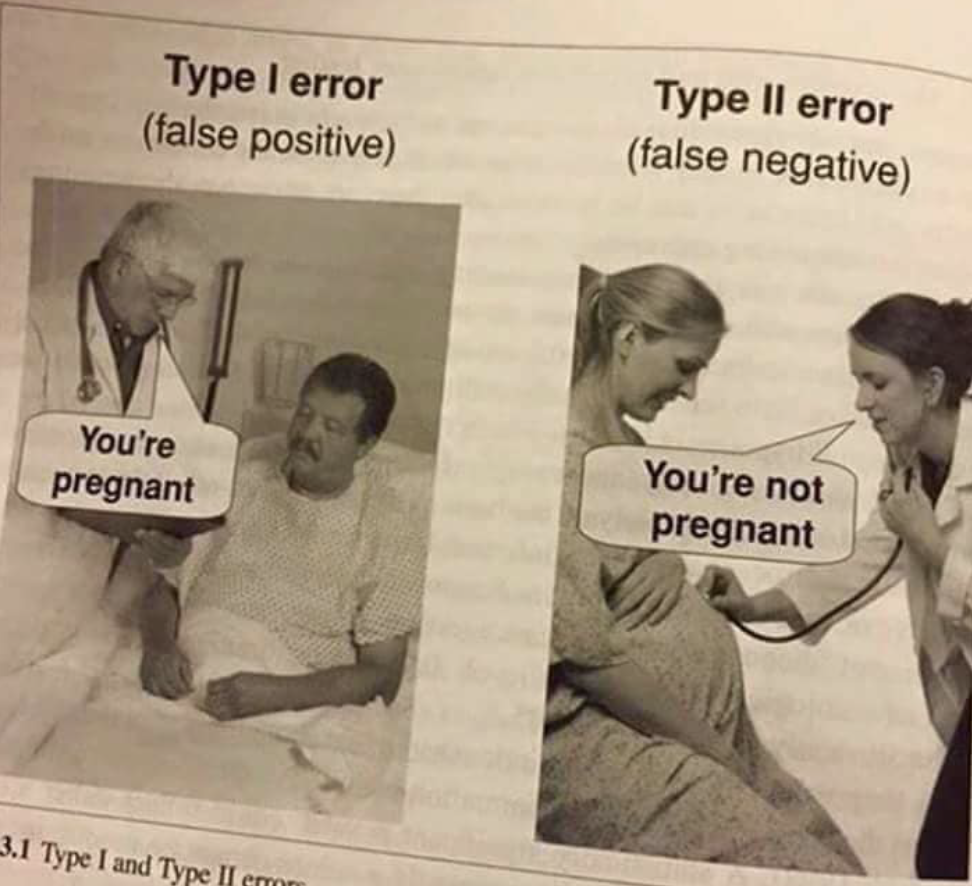
\includegraphics[width=0.45\tw]{22/error-types.png}
%\end{center}

%\end{multicols}

\clearpage

\bb[resume]
\ii A hospital is testing to see whether a donated organ is a match for a recipient in need of an organ transplant. $H_0$ would be the claim that the organ is not a match (boring). $H_a$ would be the claim that the organ is a match (interesting). Describe the Type I and Type II errors in this context. What are the practical consequences of making these errors?

\vfill

\ii A lab runs viral tests to see whether a person is currently infected with COVID-19. $H_0$ would be the claim that a person is not currently infected with COVID-19 (boring). $H_a$ would be the claim that a person is currently infected with COVID-19 (interesting). Describe the Type I and Type II errors in this context. What are the practical consequences of making these errors?

\vfill

\ii If the cholesterol level of healthy men is normally distributed with a mean of 180 and a standard deviation of 20,whereas
men predisposed to heart disease have a mean cholesterol level of 300 with a standard deviation of 30, and
The cholesterol level 225 is used to demarcate healthy from predisposed men. %It is known that 90\% of men have healthy cholesterol levels (so 10\% are predisposed).

\bb
\ii Given that a man is healthy, what is the probability they are diagnosed as predisposed? \vfill
\ii Given that a man is not healthy, what is the probability they are not diagnosed as predisposed? \vfill
\ii Which of the previous answers gives the probability of Type I error and which is for Type II error? Explain. \vspace{1in}
\ee


\clearpage

\begin{center}
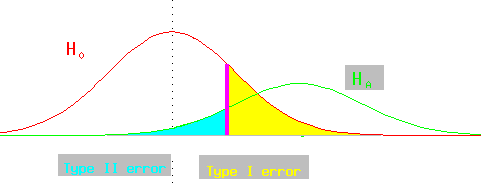
\includegraphics[width=0.75\tw]{22/fig-dist-error-types.png}
\end{center}


\ii Suppose we want to test whether a ten-sided die is fair (with sides numbered 0 to 9). Let $p$ be the proportion of all rolls that land on an even number.
\bb
\ii Set up the hypotheses. \vspace{1.5in}
\ii Roll the die 20 times, and record how many times it lands on an even number (0, 2, 4, 6, or 8). \vspace{1in}
\ii Calculate the P-value of your sample. \vfill
\ii What (if anything) can you conclude about the hypothesis at 10\% significance level? \vspace{1.5in}
\ee
\ee

\bbox
The \textbf{\colorb{significance level}} of a hypothesis test is therefore the largest value of $\alpha$ we find acceptable for the probability for a Type I error.
\ebox


